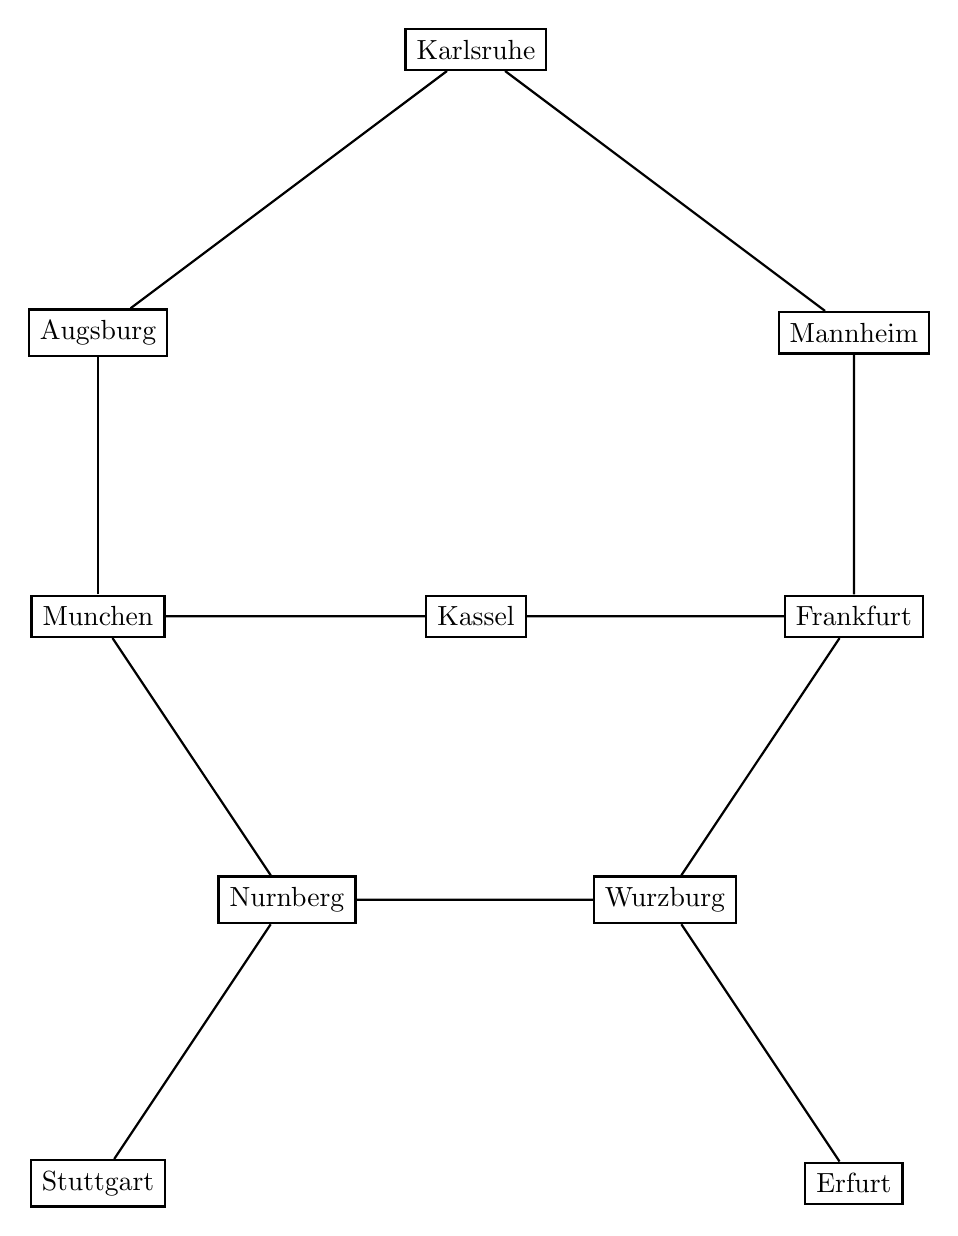
\begin{tikzpicture}
[nodedecorate/.style={shape=rectangle,inner sep=4pt,draw,thick},%
 linedecorate/.style={-,thick},%
 scale=1.2]
%% nodes or vertices
\foreach \nodename/\x/\y in {Stuttgart/0/0, Erfurt/8/0, Nurnberg/2/3,
 Wurzburg/6/3, Munchen/0/6, Frankfurt/8/6, Kassel/4/6, Augsburg/0/9,
 Mannheim/8/9, Karlsruhe/4/12}
{
  \node (\nodename) at (\x,\y) [nodedecorate] {\nodename};
}
%% edges or lines
\path
\foreach \startnode/\endnode in {Stuttgart/Nurnberg, Erfurt/Wurzburg,
 Nurnberg/Wurzburg, Nurnberg/Munchen, Wurzburg/Frankfurt,
 Munchen/Kassel, Frankfurt/Kassel, Munchen/Augsburg,
 Frankfurt/Mannheim, Augsburg/Karlsruhe, Mannheim/Karlsruhe}
{
  (\startnode) edge[linedecorate] node {} (\endnode)
};
\end{tikzpicture}
